\chapter{Partial Derivatives}

\section{Functions of Several Variables}
A function $f$ of two variables is a rule that assigns to each ordered pair of
real numbers $(x,y)$ in a set $D$ a unique real number denoted by
$f(x,y)$. The set $D$ is the \textbf{domain} of $f$ and its \textbf{range} is
the set of values that takes on, that is, ${f(x,y)\:|\:(x,y)\in D}$.

\subsection*{Example}
Find the domains of the following functions and evaluate $f(3,2)$
\begin{enumerate}[(a)]
    \item $f(x,y)=\cfrac{\sqrt{x+y+1}}{x-1}$
    \item $f(x,y)=x\ln(y^2-x)$
\end{enumerate}

\subsection*{Solution}
\begin{enumerate}[(a)]
    \item $$f(3,2)==\frac{\sqrt{3+2+1}}{3-1}\frac{\sqrt{6}}{2}$$
          The expression for $f$ makes sense if the denominator is not 0 and the
          quantity under the square root sign is nonnegative. So the domain of $f$ is
          $$D=\{(x,y)\:|\:x+y+1\geq 0, x\neq 1\}$$
          The inequality $x+y+1\geq 0$ describes the points that lie on or above the line
          $y=-x-1$, while $x\neq 1$ means that the point on the line $x=1$ must be excluded
          from the domain
    \item $$f(3,2)=3\ln(2^2-3)=3\ln(1)=0$$
          Since $\ln(y^2-x)$ is defined only when $y^2-x>0$ that is, $x<y^2$, the
          domain of $f$ is $D=\{(x,y)\:|\:x<y^2\}$. This is the set of points on the left
          of the parabola $x=y^2$.
\end{enumerate}

\subsection*{Definition}
If $f$ is a function of two variables with domain $D$, then the graph of $f$ is the
set of all points $(x,y,z)$ in $\mathbb{R}^3$ such that $z=f(x,y)$ and $(x,y)$ is in $D$

\subsection*{Example}
Sketch the graph of the function $f(x, y) = 6 - 3x - 2y$

\subsection*{Solution}
The graph of $f$ has the equation $z = 6 - 3x - 2y$, or $3x + 2y + z = 6$, which represents
a plane. To graph the plane we first find the intercepts. Putting $y = z = 0$ in the
equation, we get $x = 2$ as the $x$-intercept. Similarly, the $y$-intercept is 3 and the
$z$-intercept is 6. This helps us sketch the portion of the graph that lies in the
first octant.
\begin{center}
    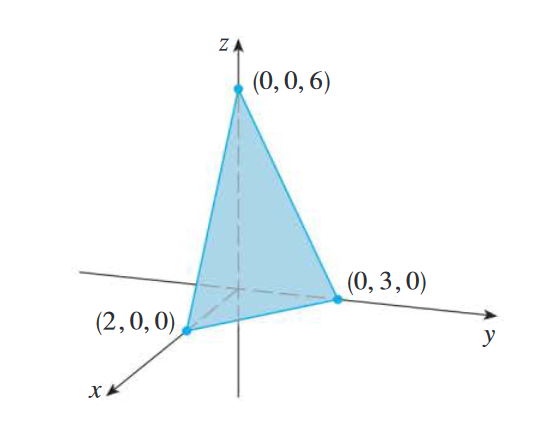
\includegraphics[scale=0.6]{example15-1-1.png}
\end{center}

\subsection*{Definition}
The level curves of a function $f$ of two variables are the curves with the equations
$f(x,y)=k$, where $k$ is a constant in the range of $f$.

\subsection*{Example}
Sketch the level curves of the function $f(x,y)=6-3x-2y$ for the values $k=-6,0,6,12$

\subsection*{Solution}
The level curves are
$$6-3x-2y=k \qquad \text{or} \qquad 3x+2y+(k-6)=0$$
This is a family of lines with slope $-\frac{3}{2}$. The four particular level curves
with $k=-6,0,6,12$ are $3x+2y-12=0$, $3x+2y-6=0$, $3x+2y=0$, and $3x+2y+6=0$. They're
equally spaced because the graph of $f$ is a plane.
\begin{center}
    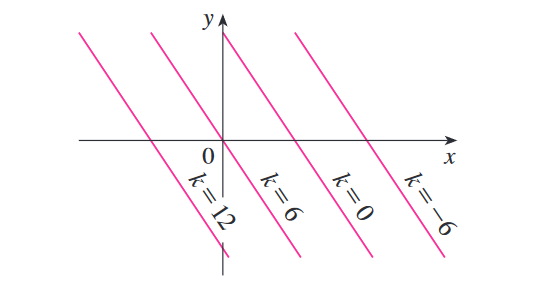
\includegraphics[scale=0.7]{example15-1-2.png}
\end{center}

\subsection*{Functions of Three or More Variables}
A \textbf{function of three variables}, $f$, is a rule that assigns to each ordered triple
$(x, y, z)$ in a domain $D\subset\mathbb{R}^3$ unique real number denoted by $f(x, y, z)$. For instance,
the temperature $T$ at a point on the surface of the Earth depends on the longitude $x$
nd the latitude y of the point and on the time $t$, so we could write $T = f(x, y, t)$.

\section{Limits and Continuity}

\subsection*{Definition}
Let $f$ be a function of two variables whose domain $D$ includes points arbitrarily
close to $(a, b)$. Then we say that the limit of $f(x, y)$ as $(x, y)$ approaches
$(a, b)$ is $L$ and we write
$$\lim_{(x,y)\to(a,b)}f(x,y)=L$$
If for every number $\epsilon>0$ there is a corresponding number $\sigma>0$ such that
if $(x,y)\in D$ and $0<\sqrt{(x-a)^2+(y-b)^2}<\delta$ and $|f(x, y) - L| < \epsilon$

\subsection*{Example}
Show that $\displaystyle\lim_{(x,y)\to(0,0)}\cfrac{x^2-y^2}{x^2+y^2}$ does not exist.

\subsection*{Solution}
Let $f(x,y)=(x^2-y^2)/(x^2+y^2)$. First let's approach (0,0) along the $x$-axis.
Then $y=0$ gives $f(x,0)=x^2/x^2=1$ for all $x\neq 0$, so
$$f(x,y)\to 1 \qquad \text{as} \qquad (x,y)\to(0,0)\quad\text{along the x-axis}$$
We now approach along the $y$-axis by putting $x=0$. Then $f(0,y)=\cfrac{-y^2}{y^2}=-1$
for all $y\neq 0$, so
$$f(x,y)\to -1 \qquad \text{as} \qquad (x,y)\to(0,0)\quad\text{along the y-axis}$$
Since $f$ has two different limits along two different lines, the limit does not exist.

\subsection*{Definition}
A function $f$ of two variables is called continuous at $(a,b)$ if
$$\lim_{(x,y)\to(a,b)} f(x,y)=f(a,b)$$
We say $f$ is continuous on $D$ if $f$ is continuous at every point $(a, b)$ in $D$.

\subsection*{Example}
Evaluate $\displaystyle\lim_{(x,y)\to(1,2)}(x^2y^3-x^3y^2+3x+2y)$

\subsection*{Solution}
Since $f(x,y)=(x^2y^3-x^3y^2+3x+2y)$ is a polynomial, it is continuous everywhere,
so we can find the limit through direct substitution:
$$\lim_{(x,y)\to(1,2)}(x^2y^3-x^3y^2+3x+2y)=(1)^2(2)^3-(1)^3(2)^2+(3)(1)+(2)(2)=11$$

\section{Partial Derivatives}
In general, if $f$ is a function of two variables $x$ and $y$, suppose we let only $x$
vary while keeping $y$ fixed, say $y = b$, where $b$ is a constant. Then we are really
considering a function of a single variable $x$, namely, $g(x) = f(x, b)$. If $g$ has
a derivative at $a$, then we call it the \textbf{partial derivative of $f$ with respect to $x$
    at $(a, b)$} and denote it by $f_x(a, b)$. Thus
$$f_x(a, b)=g'(a) \qquad \text{where} \qquad g(x) = f(x, b)$$
$$\text{which becomes} \qquad f_x(a,b)=\lim_{h\to 0}\frac{f(a+h,b)-f(a,b)}{h}$$
Similarly, the partial derivative of $f$ with respect to $y$ at $(a, b)$, denoted
by $f_y(a, b)$, is obtained by keeping $x$ fixed $(x = a)$ and finding the ordinary
derivative at $b$ of the function $G(y) = f(a, y)$:
$$f_y(a,b)=\lim_{h\to 0}\frac{f(a+h,b)-f(a,b)}{h}$$

\subsection*{Notations for Partial Derivatives}
If $z=f(x,y)$, we write
$$f_x(x,y)=f_x=\pdv{f}{x}=\frac{\partial}{\partial x}f(x,y)=\pdv{z}{x}=f_1=D_1f=D_xf$$
$$f_y(x,y)=f_y=\pdv{f}{y}=\frac{\partial}{\partial y}f(x,y)=\pdv{z}{y}=f_2=D_2f=D_yf$$

\subsection*{Rules for Finding Partial Derivatives of $z=f(x,y)$}
\begin{enumerate}
    \item To find $f_x$, regard $y$ as a constant and differentiate $f(x, y)$ with respect to $x$
    \item To find $f_y$, regard $x$ as a constant and differentiate $f(x, y)$ with respect to $y$
\end{enumerate}

\subsection*{Example}
If $f(x, y)  = x^3+x^2y^3-2y^2$, find $f_x(2, 1)$ and $f_y(2, 1)$

\subsection*{Solution}
Holding $y$ cosntant and differentiating with respect to $x$, we get
$$f_x(x,y)=3x^2+2xy^3$$
$$f_x(2,1)=3\cdot 2^2+2\cdot 2\cdot 1^3=16$$
Holding $x$ constant and differentiating with respect to $y$, we get
$$f_y(x,y)=3x^2y^2-4y$$
$$f_y(2,1)=3\cdot 2^2\cdot 1^2-4\cdot 1=8$$

\subsection*{Example}
Find $\partial z/\partial x$ and find $\partial z/\partial y$ if $z$ is defined implicitly
as a function $x$ and $y$ by the equation
$$x^3+y^3+z^3+6xzy=1$$

\subsection*{Solution}
To find $\partial z/\partial x$, we differentiate implicitly with respect to $x$,
being careful to treat $y$ as a constant:
$$3x^2+3z^2\pdv{z}{x}+6yz+6xy\pdv{z}{x}=0$$
Solving this equation for $\partial z/\partial x$, we obtain
$$\pdv{z}{x}=-\frac{x^2+2yz}{z^2+2xy}$$
Similarly, implicit differentiation with respect to $y$ gives
$$\pdv{z}{y}=-\frac{y^2+2xz}{z^2+2xy}$$

\subsection*{Higher Derivatives}
If $f$ is a function of two variables, then its partial derivatives $f_x$ and $f_y$
are also functions of two variables, so we can consider their partial derivatives
$(f_x)_x$, $(f_x)_y$, $(f_y)_x$, and $(f_y)_y$, which are called the \textbf{second
    partial derivatives} of $f$. If $z=f(x,y)$, we use the following notation:
\begin{center}
    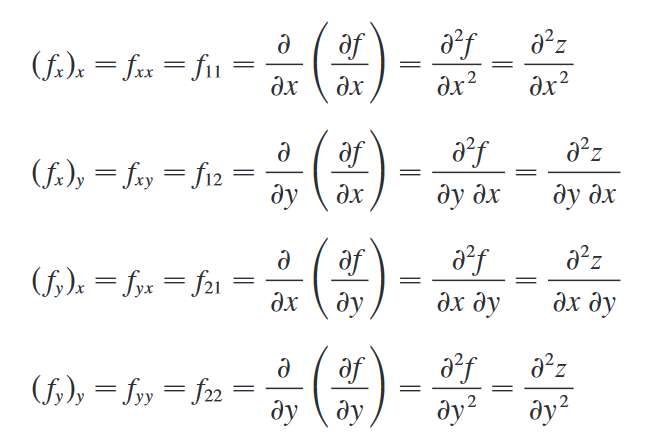
\includegraphics[scale=0.6]{example15-3-1.png}
\end{center}

\subsection*{Clairaut's Theorem}
Suppose $f$ is defined on a disk $D$ that contains the point $(a, b)$.
If the functions $f_{xy}$ and $f_{yx}$ are both continuous on D, then
$f_{xy}(a, b)$ = $f_{yx}(a, b)$

\subsection*{Example}
Calculate $f_{xxyz}$ if $f(x, y, z) = sin(3x + yz)$
\begin{enumerate}
    \item[] $f_x = 3cos(3x + yz)$
    \item[] $f_{xx} = -9sin(3x + yz)$
    \item[] $f_{xxy} = -9zcos(3x + yz)$
    \item[] $f_{xxyz} = -9cos(3x + yz) + 9yzsin(3x + yz)$
\end{enumerate}

\section{Tangent Planes and Linear Approx}
Suppose $f$ has continuous partial derivatives. An equation of the tangent plane
to the surface $z = f(x, y)$ at the point $P(x_o, y_o, z_o)$ is
$$z-z_0=f_x(x_0,y_0)(x-x_0)+f_y(x_0,y_0)(y-y_0)$$

\subsection*{Example}
Find the tangent plane to the elliptic paraboloid $z=2x2+y2$ at the point $(1, 1, 3)$.

\subsection*{Solution}
Let $f(x, y) =  2x^2 + y^2$. Then
$$f_x(x, y) = 4x \qquad f_y(x, y) = 2y$$
$$f_x(1, 1) = 4 \qquad f_y(1, 1) = 2$$
The equation of the tangent plane at $(1, 1, 3)$ is
$$z - 3 = 4(x - 1) + 2(y - 1)$$
$$\text{or} \qquad z = 4x + 2y - 3$$
Figure (a) shows the elliptic paraboloid and its tangent plane at $(1,1,3)$. Figures
(b) and (c) are zoomed in towards the point $(1,1,3)$. The more we zoom, the flatter the graph appears.
\begin{center}
    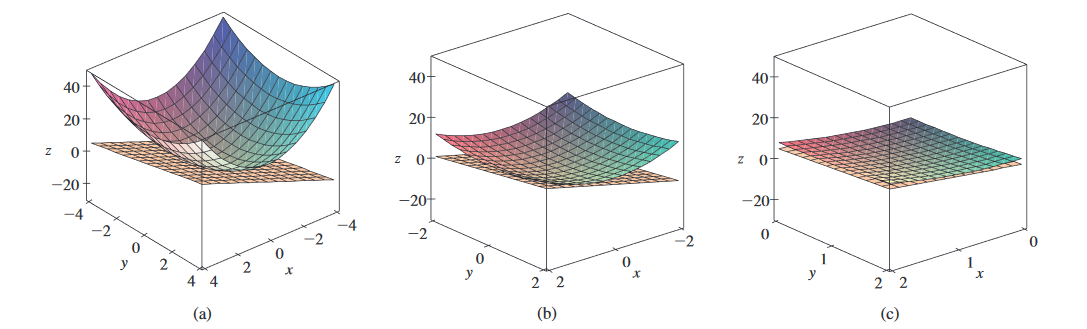
\includegraphics[scale=0.5]{example15-4-1.png}
\end{center}

\subsection*{Definition}
If $z=f(x,y)$, then $f$ is differentiable at $(a,b)$ if $\Delta z$ can be expressed
in the form
$$\Delta z=f_x(a,b)\Delta x+f_y(a,b)\Delta y+\epsilon_1\Delta x+\epsilon_2\Delta y$$
Where $\epsilon_1$ and $\epsilon_2 \to 0$ as $(\Delta x, \Delta y)\to(0,0)$

\subsection*{Theorem}
If the partial derivatives $f_x$ and $f_y$ exist near $(a, b)$ and are continuous at
$(a, b)$ then $f$ is differentiable at $(a, b)$.

\subsection*{Differentials}
For a differentiable function of two variables $z = f(x, y)$, we define the
\textbf{differentials} $dx$ and $dy$ to be independent variables; that is, they can be
given any values. Then the \textbf{differential} $dz$, also called
the \textbf{total differential}, is defined by
$$dz = f_x(x, y) dx + f_y(x, y) dy = \pdv{z}{x}dx + \pdv{z}{y}dy$$

\subsection*{Example}
\begin{enumerate}[(a)]
    \item If $z=f(x,y)=x^2+3xy-y^2$, find the differential $dz$.
    \item If $x$ changes from 2 to 2.05 and $y$ changes from 3 to 2.96, compare the values of $\Delta z$ and $dz$.
\end{enumerate}

\subsection*{Solution}
\begin{enumerate}[(a)]
    \item $$dz=\pdv{z}{x}dx+\pdv{z}{y}dy=(2x+3y)dx+(3x-2y)dy$$
    \item Putting $x=2$, $dx=\Delta x=0.05$, $y=3$, and $dy=\Delta y=-0.04$, we get
          $$dz=[2(2)+3(3)](0.05)+[3(2)-2(3)](-0.04)=0.65$$
\end{enumerate}
The increment of $z$ is
$$\Delta z=f(2.05,2.96)-f(2,3)$$
$$=[(2.05)^2+3(2.05)(2.96)-(2.96)^2]-[2^2+3(2)(3)-3^2]=6.449$$

\section{The Chain Rule}

\subsection*{The Chain Rule (Case 1)}
Suppose that $z = f(x, y)$ is a differentiable function of $x$ and $y$, where
$x = g(t)$ and $y = h(t)$ are both differentiable functions of $t$. Then
$z$ is a differentiable function of $t$ and
$$\dv{z}{t}=\pdv{f}{x}\dv{x}{t}+\pdv{f}{y}\dv{y}{t}$$

Since we often write $\pdv{z}{x}$ in place of $\pdv{f}{x}$, we can rewrite the Chain
Rule in the form
$$\dv{z}{t}=\pdv{z}{x}\dv{x}{t}+\pdv{z}{y}\dv{y}{t}$$

\subsection*{Example}
The pressure $P$ (in kilopascals), volume $V$ (in liters), and temperature $T$
(in kelvins) of a mole of an ideal gas are related by the equation $PV=8.31T$. Find
the rate at which pressure is chaning when the temperature is 300 K and increasing at
a rate of 0.1 K/s and the volume is 100 L and increasing at a rate of 0.2 L/s.

\subsection*{Solution}
If $t$ represents the time elapsed in seconds, then at the given instant we have
$T=300$, $\dv{T}{t}=0.1$, $V=100$, and $\dv{V}{t}=0.2$. Since
$$P=8.31\frac{T}{V}$$
the Chain Rule gives
$$\dv{P}{t}=\pdv{P}{T}\dv{T}{t}+\pdv{P}{V}\dv{V}{t}=\frac{8.31}{V}\dv{T}{t}-
    \frac{8.31T}{V^2}\dv{V}{t}$$
$$=\frac{8.31}{100}(0.1)-\frac{8.31(300)}{100^2}(0.2)=-0.04155$$
The pressure is decreasing at a rate of about 0.042 kPa/s.

We now consider the situation where $z=f(x,y)$ but each of $x$ and $y$ is a function
of two variables $s$ and $t$: $x=g(s,t)$, $y=h(s,t)$. Then $z$ is indirectly a function
of $s$ and $t$ and we wish to find $\pdv{z}{s}$ and $\pdv{z}{t}$. Recall that in
computing $\pdv{z}{t}$ we hold $s$ fixed and compute the ordinary derivative of $z$
with respect to $t$. Therefore,
$$\pdv{z}{t}=\pdv{z}{x}\pdv{x}{t}+\pdv{z}{y}\pdv{y}{t}$$

\subsection*{The Chain Rule (Case 2)}
Suppose that $z = f(x, y)$ is a differentiable function of $x$ and $y$, where
$x = g(s, t)$ and $y = h(s, t)$ are differentiable functions of $s$ and $t$. Then
$$\pdv{z}{s}=\pdv{z}{x}\pdv{x}{s}+\pdv{z}{y}\pdv{y}{s} \qquad
    \pdv{z}{t}=\pdv{z}{x}\pdv{x}{t}+\pdv{z}{y}\pdv{y}{t}$$

\subsection*{The Chain Rule (General Version)}
Suppose that $u$ is a differentiable function of the $n$ variables
$x_1, x_2, \dots x_n$ and each $x_j$ is a differentiable function of the $m$ variables
$t_1,t_2, \dots , t_m$ . Then $u$ is a function of $t_1,t_2, \dots , t_m$ and
$$\pdv{u}{t_i}=\pdv{u}{x_1}\pdv{x_1}{t_i}+\pdv{u}{x_2}\pdv{x_2}{t_i}+\dots+
    \pdv{u}{x_n}\pdv{x_n}{t_i}$$
for each $i=1,2,\dots ,m$.

\subsection*{Example}
If $u=x^4y+y^2z^3$, where $x=rse^t$, $y=rs^2e^{-t}$, and $z=r^2s\sin{t}$, find the
value of $\pdv{u}{s}$ when $r=2$, $s=1$, $t=0$.

\subsection*{Solution}
We have
$$\pdv{u}{s}=\pdv{u}{x}\pdv{x}{s}+\pdv{u}{y}\pdv{y}{s}+\pdv{u}{z}\pdv{z}{s}$$
$$=(4x^3y)(re^t)+(x^4+2yz^3)(2rse^{-t})+(3y^2z^2)(r^2\sin{t})$$
When $r=2$, $s=1$, and $t=0$, we have $x=2$, $y=2$, and $z=0$, so
$$\pdv{u}{s}=(64)(2)+(16)(4)+(0)(0)=192$$

\subsection*{Example}
If $g(s,t)=f(s^2-t^2,t^2-s^2)$ and $f$ is differentiable, show that $g$ satisfies
the equation
$$t\pdv{g}{s}+s\pdv{g}{t}=0$$

\subsection*{Solution}
Let $x=s^2-t^2$ and $y=t^2-s^2$. Then $g(s,t)=f(x,y)$ and the Chain Rule gives
$$\pdv{g}{s}=\pdv{f}{x}\pdv{x}{s}+\pdv{f}{y}\pdv{y}{s}=\pdv{f}{x}(2s)+\pdv{f}{y}(-2s)$$
$$\pdv{g}{t}=\pdv{f}{x}\pdv{x}{t}+\pdv{f}{y}\pdv{y}{t}=\pdv{f}{x}(-2t)+\pdv{f}{y}(2t)$$
Therefore
$$t\pdv{g}{s}+s\pdv{g}{t}=\left(2st\pdv{f}{x}-2st\pdv{f}{y}\right)+
    \left(-2st\pdv{f}{x}+2st\pdv{f}{y}\right)=0$$

\subsection*{Implicit Differentiation}
$$\dv{y}{x}=-\frac{\pdv{F}{x}}{\pdv{F}{y}}=-\frac{F_x}{F_y}$$
To derive this equation we assumed that $F(x, y) = 0$ defines $y$ implicitly as a
function of $x$. The \textbf{Implicit Function Theorem}, proved in advanced calculus,
gives conditions under which this assumption is valid. It states that if $F$ is
defined on a disk containing $(a, b)$, where $F(a, b) = 0$, $F_y(a, b)\neq 0$,
and $F_x$ and $F_y$ are continuous on the disk, then the equation $F(x, y) = 0$
defines $y$ as a function of $x$ near the point $(a, b)$ and the derivative of
this function is given by that equation.

\section{Directional Derivatives and the Gradient Vector}

\subsection*{Directional Derivatives}

\subsection*{Definition}
The \textbf{directional derivative} of $f$ at $(x_0,y_0)$ in the direction of
a unit vector $\textbf{u}=\ev{a,b}$ is
$$D_uf(x_0,y_0)=\lim_{h\to 0}\frac{f(x_0+ha,y_0+hb)-f(x_0,y_0)}{h}$$
if this limit exists.

\subsection*{Example}
Use the weather map in the figure to estimate the value of the directional derivative
of the temperature function at Reno in the southeasterly direction.

\subsection*{Solution}
The unit vector directed toward the southeast is $\mathbf{u=(i-j)}/\sqrt{2}$, but we
won't need to use this expression. We start by drawing a line through Reno toward
the southeast.
\begin{center}
    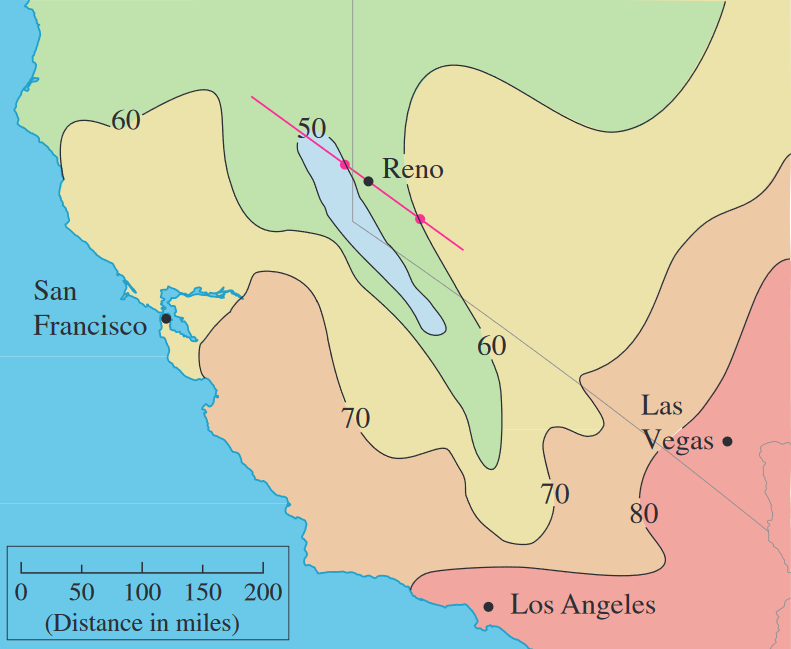
\includegraphics[scale=0.5]{example15-6-1.png}
\end{center}
We approximate the directional derivative $D_uT$ by the average rate of change of
the temperature between the points where this line intersects the isothermals
$T=50$ and $T=60$. The temperature at the point southeast of Reno is $T=60^\circ F$ and
the tempera-ture at the point northwest of Reno is $T=50^\circ F$. The distance between
these points looks to be about 75 miles. So the rate of change of the temperature
in the southeasterly direction is
$$D_uT\approx\frac{60-50}{75}=\frac{10}{75}\approx 0.13^\circ F/mi$$

\subsection*{Theorem}
If $f$ is a differentiable function of $x$ and $y$, then $f$ has a directional
derivative in the direction of any unit vector $\textbf{u}=\ev{a,b}$ and
$$D_uT=f_x(x,y)a+f_y(x,y)b$$

\subsection*{Proof}
If we define a function $g$ of the single variable $h$ by
$$g(h)=f(x_0+ha,y_0+hb)$$
then by the definition of a derivative we have
$$g'(0)=\lim_{h\to 0}\frac{g(h)-g(0)}{h}=\lim_{h\to 0}\frac{f(x_0+ha,y_0+hb)-f(x_0,y_0)}{h}$$
$$=D_uf(x_0,y_0)$$
On the other hand, we can write $g(h)=f(x,y)$, where $x=x_0+ha$, $y=y_0+hb$, so the
Chain Rule gives
$$g'(h)=\pdv{f}{x}\dv{x}{h}+\pdv{f}{y}\dv{y}{h}=f_x(x,y)a+f_y(x,y)b$$
If we now put $h=0$, then $x=x_0$, $y=y_0$, and
$$g'(0)=f_x(x_0,y_0)a+f_y(x_0,y_0)b$$
Comparing the two equations for $g'(0)$, we see that
$$D_uf(x_0,y_0)=f_x(x_0,y_0)a+f_y(x_0,y_0)b$$
If the unit vector \textbf{u} makes an angle $\theta$ with the positive $x$-axis, then
we can write $\textbf{u}=\ev{\cos{\theta},\sin{\theta}}$ and the formula in the previous theorem becomes
$$D_uf(x,y)=f_x(x,y)\cos{\theta}+f_y(x,y)\sin{\theta}$$

\subsection*{Definition}
If $f$ is a function of two variables $x$ and $y$, then the gradient of $f$ is
the vector function $\nabla f$ defined by
$$\nabla f(x,y)=\ev{f_x(x,y),f_y(x,y)}=\pdv{f}{x}\ihat\pdv{f}{y}\jhat$$

\subsection*{Definition}
The directional derivative of $f$ at $\ev{x_0, y_0, z_0}$ in the direction
of a unit vector $u = \ev{a, b, c}$ is
$$D_uf(x_0, y_0, z_0)=\lim_{h\to 0}\frac{f(x_0+ha,y_0+hb,z_0+hc)-f(x_0,y_0,z_0)}{h}$$
The compact form is
$$D_uf(x_0)=\lim_{h\to 0}\frac{f(x_0+hu)-f(x_0)}{h}$$

\subsection*{The Gradient Vector}

\subsection*{Definition}
If $f$ is a function of two variables $x$ and $y$, then the \textbf{gradient} of $f$
is the vector function $\nabla f$ defined by
$$\nabla f(x,y)=\ev{f_x(x,y),f_y(x,y)}=\pdv{f}{x}\ihat+\pdv{f}{y}\jhat$$
For a function $f$ of three variables, the \textbf{gradient vector} is
$$\nabla f=\ev{f_x,f_y,f_z}=\pdv{f}{x}\ihat+\pdv{f}{y}\jhat+\pdv{f}{z}\khat$$

\subsection*{Example}
If $f(x,y,z)=x\sin{yz}$, (a) find the gradient of $f$ and (b) find the directional
derivative of $f$ at $(1,3,0)$ in the direction of $\textbf{v}=\ihat+2\jhat-\khat$.

\subsection*{Solution}
\begin{enumerate}[(a)]
    \item The gradient of $f$ is
          $$\nabla f(x,y,z)=\ev{f_x(x,y,z),f_y(x,y,z),f_z(x,y,z)}$$
          $$=\ev{\sin{yz},cz\cos{yz},xy\cos{yz}}$$
    \item At $(1,3,0)$ we have $\nabla f(1,3,0)=\ev{0,0,3}$. The unit vector in the
          direction of $\textbf{v}=\ihat+2\jhat-\khat$ is
          $$\textbf{u}=\frac{1}{\sqrt{6}}\ihat+\frac{2}{\sqrt{6}}\jhat-\frac{1}{\sqrt{6}}\khat$$
          Therefore, $D_uf(x,y,z)=\nabla f(x,y,z) \cdot \textbf{u}$ gives us
          $$D_uf(1,3,0)=\nabla f(1,3,0)\cdot\textbf{u}$$
          $$=3\khat\cdot\left(\frac{1}{\sqrt{6}}\ihat+\frac{2}{\sqrt{6}}\jhat-\frac{1}{\sqrt{6}}\khat\right)$$
          $$=3\left(-\frac{1}{\sqrt{6}}\right)=-\sqrt{\frac{3}{2}}$$
\end{enumerate}

\subsection*{Theorem}
Suppose $f$ is a differentiable function of two or three variables. The maximum
value of the directional derivative $D_uf(x)$ is $|\nabla f(x)|$ and it occurs
when \textbf{u} has the same direction as the gradient vector $\nabla f(x)$

\subsection*{Proof}
We have
$$D_uf=\nabla f\cdot\textbf{u}=|\nabla f||\textbf{u}|\cos{\theta}=|\nabla f|\cos{\theta}$$
Where $\theta$ is the angle between $\nabla f$ and \textbf{u}. The maximum value of $\cos{\theta}$ is 1
and this occurs when $\theta = 0$. Therefore, the maximum value of $D_uf$ is $|\nabla f|$ and
it occurs when $\theta = 0$, that is, when \textbf{u} has the same direction as $\nabla f$

\section{Maximum and Minimum Values}

\subsection*{Definition}
A function of two variables has a {local maximum} at $(a, b)$ if $f(x, y)\leq f(a, b)$
when $(x, y)$ is near $(a, b)$. The number $f(a, b)$ is called a \textbf{local maximum value},
if $f(x, y)\geq f(a, b)$ when $(x, y)$ is near $(a, b)$, then $f(a, b)$ is a \textbf{local minimum value}.

\subsection*{Theorem}
If $f$ has a local maximum or minimum at $(a, b)$ and the first-order partial
derivatives of $f$ exist there, then $f_x (a, b) = 0$ and $f_y (a, b) = 0$.

\subsection*{Example}
Let $f(x,y)=x^2+y^2-2x-6y+14$. Then
$$f_(x,y)=2x-2 \qquad f_y(x,y)=2y-6$$
These partial derivatives are equal to 0 when $x=1$ and $y=3$, so the only critical
point is $(1,3)$. By completing the square, we find that
$$f(x,y)=4+(x-1)^2+(y-3)^2$$
Since $(x-1)^2\geq 0$ and $(y-3)^2\geq 0$, we have $f(x,y)\geq 4$ for all values of
$x$ and $y$. Therefore $f(1,3)=4$ is a local minimum, and in fact it is the absolute
minimum of $f$. This can be confirmed geometrically from the graph of $f$, which is the
elliptic paraboloid with vertex $(1,3,4)$.

\subsection*{Second Derivatives Test}
Suppose the second partial derivatives of $f$ are continuous on a disk with center
$(a, b)$, and suppose that $f_x (a, b) = 0$ and $f_y (a, b) = 0$ Let
$$D=D(a,b)=f_{xx}(a,b)f_{yy}(a,b)-[f_{xy}(a,b)]^2$$
\begin{enumerate}[(a)]
    \item If $D > 0$ and $f_{xx}(a, b) > 0$, then $f(a, b)$ is a local minimum
    \item If $D > 0$ and $f_{xx}(a, b) < 0$, then $f(a, b)$ is a local maximum
    \item If $D < 0$, then $f(a, b)$ is not a local maximum or minimum
\end{enumerate}

\subsection*{Example}
Find the local maximum and minimum values and saddle points of $f(x,y)=x^4+y^4-4xy+1$.

\subsection*{Solution}
We first locate the critical points:
$$f_x=4x^3-4y \qquad f_y=4y^3-4x$$
Setting these partial derivatives equal to 0, we obtain the equations
$$x^3-y=0 \qquad \text{and} \qquad y^3-x=0$$
To solve these equations we substitute $y=x^3$ from the first equation into the
second one. This gives
$$0=x^9-x=x(x^8-1)=x(x^4-1)(x^4+1)=x(x^2-1)(x^2+1)(x^4+1)$$
so there are three real roots: $x=0$, 1, -1. The three critical points are $(0,0)$,
$(1,1)$, and $(-1,-1)$. Next we calculate the second partial derivatives and $D(x,y)$:
$$f_{xx}=12x^2 \qquad f_{xy}=-4 \qquad f_{yy}=12y^2$$
$$D(x,y)=f_{xx}f_{yy}-(f_{xy})^2=144x^2y^2-16$$
Since $D(0,0)=-16<0$, it follows that form case (c) of the Second Derivatives Test that
the origin is a saddle point; that is, $f$ has no local maximum or minimum at $(0,0)$.
Since $D(1,1)=128>0$ and $f_{xx}(1,1)=12>0$, we see from case (a) of the test that
$f(1,1)=-1$ is a local minimum. Similarlym we have $D(-1,-1)=128>0$ and
$f_{xx}(-1,-1)=12>0$, so $f(-1,-1)=-1$ is also a local minimum. The graph of $f$ is shown below.
\begin{center}
    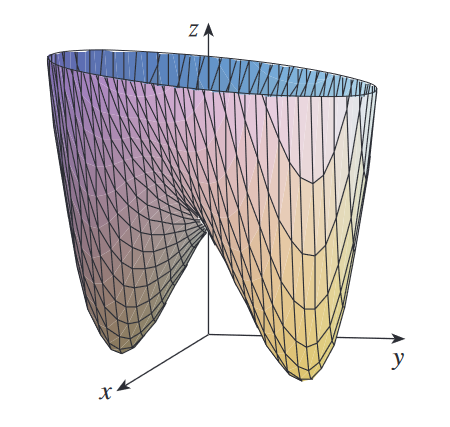
\includegraphics[scale=0.7]{example15-7-1.png}
\end{center}

\subsection*{Extreme Value Theorem for Functions of Two Variables}
If $f$ is continuous on a closed, bounded set $D$ in $\mathbb{R}^2$, then $f$
attains an absolute maximum value $f(x_1, y_1)$ and an absolute minimum value $f(x_2, y_2)$
at some points $(x_1, y_1)$ and $(x_2, y_2)$ in $D$.

To find the absolute maximum and minimum values of a continuous function $f $
on a closed, bounded set $D$:
\begin{enumerate}
    \item Find the values of $f$ at the critical points of $f$ in $D$
    \item Find the extreme values of $f$ on the boundary of $D$
    \item The largest of the values from steps 1 and 2 is the absolute maximum value;
          the smallest of these values is the absolute minimum value.
\end{enumerate}

\section{Lagrange Multipliers}

\subsection*{Method of Lagrange Multipliers}
To find the maximum and minimum values of $f(x, y, z) $subject to the
constraint $g(x, y, z) = k$:
\begin{enumerate}[(a)]
    \item Find all values of $x$, $y$, $z$, and $\lambda$ such that
          $$\nabla f(x,y,z)=\lambda\nabla g(x,y,z) \qquad \text{and} \qquad g(x,y,z)=k$$
    \item Evaluate $f$ at all points $(x, y, z)$ that result from step (a). The largest
          of these values is the maximum value of $f$; the smallest is the minimum value of $f$
\end{enumerate}

\subsection*{Example}
A rectangular box without a lid is to be made from $12\text{m}^2$ of cardboard.
Find the maximum volume of such a box.

\subsection*{Solution}
We let $x$, $y$, and $z$ be the length, width, and height, respectively, of the box in
meters. Then we wish to maximize
$$V=xyz$$
subject to the constraint
$$g(x,y,z)=2xz+2yz+xy=12$$
Using the method of lagrange multipliers, we look for values of $x$, $y$, $z$,
and $\lambda$ such that $\nabla V= \lambda\nabla g$ and $g(x, y, z) = 12$. This gives the equations
$$V_x=\lambda g_x \qquad V_y=\lambda g_y \qquad V_z=\lambda g_z \qquad 2xz+2yz+xy=12$$
which become
\begin{enumerate}
    \item[(2)] $yz=\lambda(2z+y)$
    \item[(3)] $xz=\lambda(2z+x)$
    \item[(4)] $xy=\lambda(2x+2y)$
    \item[(5)] $2xz+2yz+xy=12$
\end{enumerate}
There are no general rules for solving systems of equations. Sometimes ingenuity
is required. In the present example you might notice that if we multiply (2)
by $x$, (3) by $y$, and (4) by $z$, then the left sides of these equations will be
identical. We get
\begin{enumerate}
    \item[(6)] $xyz=\lambda(2xz+xy)$
    \item[(7)] $xyz=\lambda(2yz+xy)$
    \item[(8)] $xyz=\lambda(2xz+2yz)$
\end{enumerate}
We observe that $\lambda$ is  not equal to 0 because $\lambda = 0$ would imply
$yz - xz - xy = 0$. From (2), (3), and (4) and this would contradict (5).
Therefore, from (6) and (7) we have
$$2xz+xy=2yz+xy$$
which gives $xz=yz$. But $z\neq 0$ (since $z=0$ would give $V=0$), so $x=y$.
From (7) and (8) we have
$$2yz+xy=2xz+2yz$$
which gives $2xz=xy$ and so (since $x\neq 0$) $y=2z$. If we now put $x=y=2z$ in (5), we get
$$4z^2+4z^2+4z^2=12$$
Since $x$, $y$, and $z$ are all positive, we therefore have $z=1$ and so $x=2$ and $y=2$.

\subsection*{Example}
Find the maximum value of the function $f(x,y,z)=x+2y+3z$ on the curve of the
intersection of the plane $x-y+z=1$ and the cylinder $x^2+y^2=1$.

\subsection*{Solution}
We maximum the function $f(x,y,z)=x+2y+3z$ subject to the constraints $g(x,y,z)=x-y+z=1$
and $h(x,y,z)=x^2+y^2=1$. The Lagrange condition is $\nabla f=\lambda\nabla g+\mu\nabla h$,
so we solve the equations
\begin{enumerate}
    \item[(17)] $1=\lambda+2x\mu$
    \item[(18)] $2=-\lambda+2y\mu$
    \item[(19)] $3=\lambda$
    \item[(20)] $x-y+z=1$
    \item[(21)] $x^2+y^2=1$
\end{enumerate}
Putting $\lambda=3$ /[from (19)/] in (17), we get $2x\mu=-2$, so $x=-1/\mu$. Similarly,
(18) gives $y=5/(2\mu)$. Substitution in (21) then gives
$$\frac{1}{\mu^2}+\frac{25}{4\mu^2}=1$$
and so $\mu^2=\frac{29}{4}$, $\mu=\pm\sqrt{29}/2$. Then $x=\mp 2/sqrt{29}$,
$y=\pm 5/\sqrt{29}$, and, from (2), $z=1-x+y=1\pm 7/\sqrt{29}$. The corresponding values of $f$ are
$$\mp\frac{2}{\sqrt{29}}+2\left(\pm\frac{5}{\sqrt{29}}\right)+3\left(1\pm\frac{7}{\sqrt{29}}\right)=
    3\pm\sqrt{29}$$
Therefore, the maximum value of $f$ on the given curve is $3+\sqrt{29}$.